%
% FH Technikum Wien
% !TEX encoding = UTF-8 Unicode
%
% Erstellung von Master- und Bachelorarbeiten an der FH Technikum Wien mit Hilfe von LaTeX und der Klasse TWBOOK
%
% Um ein eigenes Dokument zu erstellen, müssen Sie folgendes ergänzen:
% 1) Mit \documentclass[..] einstellen: Master- oder Bachelorarbeit, Studiengang und Sprache
% 2) Mit \newcommand{\FHTWCitationType}.. Zitierstandard festlegen (wird in der Regel vom Studiengang vorgegeben - bitte erfragen)
% 3) Deckblatt, Kurzfassung, etc. ausfüllen
% 4) und die Arbeit schreiben (die verwendeten Literaturquellen in Literatur.bib eintragen)
%
% Getestet mit TeXstudio mit Zeichenkodierung ISO-8859-1 (=ansinew/latin1) und MikTex unter Windows
% Zu beachten ist, dass die Kodierung der Datei mit der Kodierung des paketes inputenc zusammen passt!
% Die Kodierung der Datei twbook.cls MUSS ANSI betragen!
% Bei der Verwendung von UTF8 muss dnicht nur die Kodierung des Dokuments auf UTF8 gestellt sein, sondern auch die des BibTex-Files!
%
% Bugreports und Feedback bitte per E-Mail an latex@technikum-wien.at
%
% Versionen
% *) V0.7: 9.1.2015, RO: Modeline angepasst und verschoben
% *) V0.6: 10.10.2014, RO: Weitere Anpassung an die UK
% *) V0.5: 8.8.2014, WK: Literaturquellen überarbeitet und angepasst
% *) V0.4: 4.8.2014, WK: Initalversion in SVN eingespielt
%
\documentclass[Bachelor,BIF,english]{twbook}
\usepackage[utf8]{inputenc}
\usepackage[T1]{fontenc}

%
% Bitte in der folgenden Zeile den Zitierstandard festlegen
\newcommand{\FHTWCitationType}{IEEE} % IEEE oder HARVARD möglich - wenn Sie zwischen IEEE und HARVARD wechseln, bitte die temorären Dateien (aux, bbl, ...) löschen
%
\ifthenelse{\equal{\FHTWCitationType}{HARVARD}}{\usepackage{harvard}}{\usepackage{bibgerm}}

% Definition Code-Listings Formatierung:
\usepackage[final]{listings}
\lstset{captionpos=b, numberbychapter=false,caption=\lstname,frame=single, numbers=left, stepnumber=1, numbersep=2pt, xleftmargin=15pt, framexleftmargin=15pt, numberstyle=\tiny, tabsize=3, columns=fixed, basicstyle={\fontfamily{pcr}\selectfont\footnotesize}, keywordstyle=\bfseries, commentstyle={\color[gray]{0.33}\itshape}, stringstyle=\color[gray]{0.25}, breaklines, breakatwhitespace, breakautoindent}
\lstloadlanguages{[ANSI]C, C++, [gnu]make, gnuplot, Matlab}

%Formatieren des Quellcodeverzeichnisses
\makeatletter
% Setzen der Bezeichnungen für das Quellcodeverzeichnis/Abkürzungsverzeichnis in Abhängigkeit von der eingestellten Sprache
\providecommand\listacroname{}
\@ifclasswith{twbook}{english}
{%
    \renewcommand\lstlistingname{Code}
    \renewcommand\lstlistlistingname{List of Code}
    \renewcommand\listacroname{List of Abbreviations}
}{%
    \renewcommand\lstlistingname{Quellcode}
    \renewcommand\lstlistlistingname{Quellcodeverzeichnis}
    \renewcommand\listacroname{Abkürzungsverzeichnis}
}
% Wenn die Option listof=entryprefix gewählt wurde, Definition des Entyprefixes für das Quellcodeverzeichnis. Definition des Macros listoflolentryname analog zu listoflofentryname und listoflotentryname der KOMA-Klasse
\@ifclasswith{scrbook}{listof=entryprefix}
{%
    \newcommand\listoflolentryname\lstlistingname
}{%
}
\makeatother
\newcommand{\listofcode}{\phantomsection\lstlistoflistings}

% Die nachfolgenden Pakete stellen sonst nicht benötigte Features zur Verfügung
\usepackage{blindtext}
\usepackage{parskip}

%
% Einträge für Deckblatt, Kurzfassung, etc.
%
\title{A Comparative View of Cross-compiled and Interpreted Cross-Platform Approaches for iOS and Android Mobile Application Development}
\author{Dominik Hack}
\studentnumber{1610257044}
\supervisor{Dipl.-Ing. Dr.techn. Thomas Polzer}
\place{Vienna}
\kurzfassung{Heutzutage fällt die Entscheidung in den meisten Fällen auf platformspezifische Frameworks für die Entwicklung einer mobilen Applikation. Jedoch bedeutet das, dass für jede Platform eine neue Applikation entwickelt werden muss. Abhilfe dafür würden Cross-Platform Frameworks schaffen, welche trotz nur einer Codebasis auf allen unterstützten Platformen eine ausführbare Applikation erzeugen können, weswegen sich diese Arbeit diesem Thema widmet.
Im ersten Teil werden  die Stärken und Schwächen mobiler Cross-Platform Entwicklungsmethoden vorgestellt. Im zweiten Teil findet eine Gegenüberstellung von zwei Cross-Platform Frameworks mit verschiedenen Entwicklungsmethoden anhand von der Ausarbeitung von mehreren Studien statt. Dabei wurde sich im Detail auf die beiden Entwicklungsmethoden cross-compiled und interpreted konzentriert und daher wurde pro Entwicklungsmethode ein Cross-Platform Famework gewählt, welches jene Methode verwendet. In diesem Fall fiel die Wahl auf Xamarin sowie auf React Native. Bei der Evaluierung der beiden Frameworks in Bezug auf Unterschiedlichkeiten sowohl untereinander als auch im Vergleich zu platformspezifischen Frameworks richtet sich das Augenmerk auf die Kriterien Performance, Code Sharing, Dokumentation und Look and feel. Durch die ausgearbeiteten Resultate der Studien zeigt sich, dass Cross-Platform Frameworks den platformspezifischen Frameworks an fast nichts mehr nachliegen und manchmal sogar bessere Ergebnisse vorweisen können.}
\schlagworte{Platformübergreifende Entwicklung, Xamarin, React Native, Mobile Software Entwicklung}
\outline{Today, most companies choose to use platform-specific frameworks when developing a mobile application, although this means, that they need to develop separate applications for each supported platform. A possible solution for this would be the use of cross-platform frameworks which can generate an executable application on all supported platforms in spite of just one code base. Which is why this thesis is devoted to this topic.
In the first part strengths and weaknesses of mobile cross-platform development approaches are introduced and analyzed. In the second part, a comparison of two cross-platform frameworks with different development approaches based on the preparation of several studies takes place. As the focus of this part lies on two development approaches, cross-compiled and interpreted, a cross-platform framework for each development approach was chosen in order to allow comparison between both approaches more easily. In this case, the choice fell on Xamarin and React Native. While evaluating the two frameworks in terms of differences between each other as well as compared to platform-specific frameworks, four key criteria were chosen: performance, code sharing, documentation and look and feel. The results of the studies show that cross-platform frameworks perform on an almost equal and sometimes even higher level as platform-specific frameworks.}
\keywords{Cross-Platform Development, Xamarin, React Native, Mobile Software Development}

\begin{document}

%Festlegungen für den HARVARD-Zitierstandard
\ifthenelse{\equal{\FHTWCitationType}{HARVARD}}{
\bibliographystyle{Harvard_FHTW_MR}%Zitierstandard FH Technikum Wien, Studiengang Mechatronik/Robotik, Version 1.2e
\citationstyle{dcu}%Correct citation-style (Harvardand, ";" between citations, "," between author and year)
\citationmode{abbr}%use "et al." with first citation
\iflanguage{ngerman}{
    %Deutsch Neue Rechtschreibung
    \newcommand{\citepic}[1]{(Quelle: \protect\cite{#1})}%Zitat: Bild
    \newcommand{\citefig}[2]{(Quelle: \protect\cite{#1}, S. #2)}%Zitat: Bild aus Dokument
    \newcommand{\citefigm}[2]{(Quelle: modifiziert "ubernommen aus \protect\cite{#1}, S. #2)}%Zitat: modifiziertes Bild aus Dokument
    \newcommand{\citep}{\citeasnoun}%In-Line Zitiat entweder mit \citep{} oder \citeasnoun{}
    \newcommand{\acessedthrough}{Verf{\"u}gbar unter:}%Für URL-Angabe
    \newcommand{\acessedthroughp}{Verf{\"u}gbar bei:}%Für URL-Angabe (Geschützte Datenbank, Zugriff durch FH)
    \newcommand{\acessedat}{Zugang am}%Für URL-Datum-Angabe
    \newcommand{\singlepage}{S.}%Für Seitenangabe (einzelne Seite)
    \newcommand{\multiplepages}{S.}%Für Seitenangabe (mehrere Seiten)
    \newcommand{\chapternr}{K.}%Für Kapitelangabe
    \renewcommand{\harvardand}{\&}%Harvardand in Zitaten
    \newcommand{\abstractonly}{ausschließlich Abstract}
    \newcommand{\edition}{. Auflage}%Angabe der Auflage
}{
\iflanguage{german}{
    %Deutsch
    \newcommand{\citepic}[1]{(Quelle: \protect\cite{#1})}%Zitat: Bild
    \newcommand{\citefig}[2]{(Quelle: \protect\cite{#1}, S. #2)}%Zitat: Bild aus Dokument
    \newcommand{\citefigm}[2]{(Quelle: modifiziert "ubernommen aus \protect\cite{#1}, S. #2)}%Zitat: modifiziertes Bild aus Dokument
    \newcommand{\citep}{\citeasnoun}%In-Line Zitiat entweder mit \citep{} oder \citeasnoun{}
    \newcommand{\acessedthrough}{Verf{\"u}gbar unter:}%Für URL-Angabe
    \newcommand{\acessedthroughp}{Verf{\"u}gbar bei:}%Für URL-Angabe (Geschützte Datenbank, Zugriff durch FH)
    \newcommand{\acessedat}{Zugang am}%Für URL-Datum-Angabe
    \newcommand{\singlepage}{S.}%Für Seitenangabe (einzelne Seite)
    \newcommand{\multiplepages}{S.}%Für Seitenangabe (mehrere Seiten)
    \newcommand{\chapternr}{K.}%Für Kapitelangabe
    \renewcommand{\harvardand}{\&}%Harvardand in Zitaten
    \newcommand{\abstractonly}{ausschließlich Abstract}
    \newcommand{\edition}{. Auflage}%Angabe der Auflage
}{
    %Englisch
    \newcommand{\citepic}[1]{(Source: \protect\cite{#1})}%Zitat: Bild
    \newcommand{\citefig}[2]{(Source: \protect\cite{#1}, p. #2)}%Zitat: Bild aus Dokument
    \newcommand{\citefigm}[2]{(Source: taken with modification from \protect\cite{#1}, p. #2)}%Zitat: modifiziertes Bild aus Dokument
    \newcommand{\citep}{\citeasnoun}%In-Line Zitiat entweder mit \citep{} oder \citeasnoun{}
    \newcommand{\acessedthrough}{Available at:}%Für URL-Angabe
    \newcommand{\acessedthroughp}{Available through:}%Für URL-Angabe (Geschützte Datenbank, Zugriff durch FH)
    \newcommand{\acessedat}{Accessed}%Für URL-Datum-Angabe
    \newcommand{\singlepage}{p.}%Für Seitenangabe (einzelne Seite)
    \newcommand{\multiplepages}{pp.}%Für Seitenangabe (mehrere Seiten)
    \newcommand{\chapternr}{Ch.}%Für Kapitelangabe
    \renewcommand{\harvardand}{\&}%Harvardand in Zitaten
    \newcommand{\abstractonly}{Abstract only}
    \newcommand{\edition}{~edition}%Edition -> note, that you have to write "edition = {2nd},"!
}}}

\maketitle

\chapter{Introduction}
Almost everyone owns a smartphone these days: according to studies from 2017, 2 billion of these devices were in circulation worldwide \cite[p.~184]{MartinezLecomte2017}. As more and more companies realize the importance of smartphones, so does the demand for mobile applications for their worker's or customer’s smartphones and as a result, more developers are needed for mobile application development \cite{Danielsson_2016} \cite{GaouarBenamarBendimerad2016}.
However, certain mobile applications do not run on every mobile device. According to a study \cite{OSMarketShare} from 2018, 86.8\% of smartphones worldwide use Android (Google LLC, Mountain View CA) and 13.2\% iOS (Apple Inc., Cupertino CA) \cite[p.~5]{Steczko2016}. This means, that an App-developer  would have to develop a separate application for each supported platform and for most of the history of app development, this was the standard way to go. Because the first solutions for cross-platform development were based only on web development, applications ran with significantly lower performance levels, had no way to use any hardware features of the respective devices and were only accessible via an internet browser \cite[p.~626]{6420693} \cite[p.~1]{7934674}.
\\[\baselineskip]
However, a lot has changed since then. Now, there are different approaches to this problem besides developing a web application. Almost every one of these approaches is based on some mature frameworks that have already been tested by various researchers through several studies Latif, Lakhrissi, Nfaoui and Es-Sbai published a paper \cite{7479278} in which they summarized all mobile cross platform development approaches and compared them with each other. As a result of their analysis they identified a multitude of desirable requirements, any cross-platform technology should fulfill. These requirements are: application scalability and maintainability, access to features of device, auto-optimization of resource consumption, security and a development environment that features intelligent auto-completion systems, debuggers, compilers and simulators for all supported platforms. Another paper \cite{7934674} published by the same authors also discusses mobile cross-platform development approaches but concentrates on comparing frameworks based on the aforementioned approaches. In the following chapters of this thesis these mobile development approaches will be explained further and the benefits along with the disadvantages of each will be listed.
\\[\baselineskip]
Furthermore, by analyzing, summarizing and comparing the results of studies regarding the frameworks Xamarin and React Native, the potential of the interpreted approach and the cross-compiled approach will also be discussed in the following chapters. An example of such studies would be the paper of Jesper Söderberg and Erik Johansson in which they implemented a React Native (Facebook Inc., Menlo Park CA) feature set (e.g. scrollable list, screen transition, background process, native module) and analyzed it through performance parameters such as CPU and GPU usage to showcase that even though a native application has still better performance the difference is not very large and therefore can be ignored for most applications \cite{JohanssonSderberg2018}. Another example would be Marc Armgren’s paper, in which he compared a Xamarin (Microsoft Corporation, Redmond WA) application with native applications by running user interface, computational and network benchmark tests \cite{Armgren_2015}. In his paper, Armgen showcased, that applications with a high value on the user interface or frequent requests of data from the network without high computing power requirements can be implemented on Xamarin. In the computational benchmark tests, however, the native applications led Marc Armgren to the conclusion that Xamarin’s cross-compiler was not yet as optimized as the compilers for the native applications \cite{Armgren_2015}.
\\[\baselineskip]
In this thesis, various noteworthy results of papers, studies and theses (\cite{Danielsson_2016}, \cite{Hansson_Vidhall_2016}, \cite{MartinezLecomte2018}, \cite{ZubaBernhard2017EdPb}, \cite{WillocxVossaertNaessens2015}, \cite{MartinezLecomte2017}, \cite{Dickson_2013}, \cite{GaouarBenamarBendimerad2016}, \cite{7479278}, \cite{LinckArne2016}, \cite{7934674}) that either experiment with Xamarin or React Native or both will be summarized and their results presented. Besides performance, this thesis will also include other criteria such as code sharing, documentation and look and feel. If possible, the results of each criteria will contain a discussion comparing Xamarin and React Native with each other. 
\\[\baselineskip]
The following research questions will be the focus of this thesis:
\begin{itemize}
\item Does an application developed in Xamarin perform as well as one developed in React Native and which one performs better compared to a native application created in Android or iOS?
\item How much code from an application written using Xamarin or React Native can be shared between Android and iOS?
\item Do the documentations of Xamarin and React Native lack information needed to develop features?
\item Will the look and feel of a native application created in Xamarin or React Native adhere to the OS user interface guidelines?
\end{itemize}

\newpage
\chapter{Mobile Development Approaches}
To this day, lots of companies, if not all of them, realized that offering mobile applications on smartphones or other mobile devices to their customers is crucial for asserting themselves against the competition \cite{7479278}. If a company chooses to provide a mobile application for their customers, they do not want to offer the mobile application to only half of them. However, to equally provide all customers with the same service, a company has to develop their mobile application for multiple platforms \cite[p.~5]{Steczko2016}.
\\[\baselineskip]
Nevertheless, without precisely planning the development and maintenance of multiple mobile applications for various platforms the company may invest more money into the development and maintenance than necessary \cite[p.~757]{Ciman2014} \cite[p.~1]{JohanssonSderberg2018} \cite[p.~8]{Steczko2016}. One of the things to consider is what framework should be used for the development of the application. There are lots of frameworks for mobile application development out there and nearly every framework was built by applying one mobile development approach. Each approach has different advantages and disadvantages; thus the usefulness of each approach is highly dependent of the situation it is used in \cite{7934674} \cite{6420693}. This means in order to minimize costs and thereby increase the chance of the project’s success, it is essential to choose a framework with a suitable mobile development approach for the given situation. To assist in finding the most valuable approach for each project, the following sections summarize the most used mobile development approaches. 

\section{Native Approach}
Choosing the native development approach implicates developing the same application separately for each platform it should be available on. Usually the most commonly used platforms on the market, which to this day are Android and iOS, are chosen to be supported \cite[p.~5]{Steczko2016}. As a result, at least two applications have to be developed every time: one for Android by using the Android-SDK and Java as the programming language, and one for iOS by using the iOS-SDK and Swift as the programming language \cite[p.~5]{LinckArne2016} \cite{AppleGettingStarted}. Even though this leads to the requirement of different skill sets and therefore potentially more developers being necessary for the development of the application, it also leads to applications developed by utilizing the official platform specific frameworks and tools recommended by the publishers of the platforms. 
\\[\baselineskip]
Through using platform specific frameworks and tools, a developer is able to directly communicate with the operating system of the mobile device. This allows the developer to get access to features like sensors or cloud services without having to rely on other, potentially performance-decreasing alternatives, cross-platform applications would otherwise have to use in order to communicate with the operating system and get access to the previously mentioned features \cite[p.~6]{LinckArne2016}.
\\[\baselineskip]
On the downside, each application has a different code base, which means that each code base has to be maintained individually. This results in two, generally costly consequences: Either, one developer with knowledge of developing on all platforms needs to work on maintenance for all applications or multiple developers with special knowledge regarding one specific platform have to maintain each particular platform’s application \cite[p.~6]{LinckArne2016}.

\section{Cross-Platform Approaches}
The major goal of cross-platform approaches is developing and maintaining one uniform code base for all different platforms. Additionally, other important goals include unrestricted access to all platform-dependent features and offering the same performance, impression and look and feel a native application would \cite[p.~1]{7479278} \cite[p.~1]{7934674}. To achieve these goals different solutions were developed. These solutions are the: 
\begin{itemize}
\item Using an interpreter to call native APIs at runtime \cite[p.~3]{7479278} \cite[p.~4-5]{LinckArne2016} \cite[p.~5-6]{Hansson_Vidhall_2016}.
\item Utilizing a cross-compiler to compile non-native code into a native application \cite[p.~3-4]{7479278} \cite[p.~5]{Hansson_Vidhall_2016}.
\item Developing a web application and displaying it via the browser of the mobile device \cite[p.~2]{7479278} \cite[p.~2-3]{LinckArne2016} \cite[p.~4-5]{Hansson_Vidhall_2016}.
\item Wrapping a web application into a native webview-component \cite[p.~2-3]{7479278} \cite[p.~3-4]{LinckArne2016} \cite[p.~5]{Hansson_Vidhall_2016}.
\item Working with the Model driven architecture defined by the Object Management Group to create models that will later on be transformed into native source code \cite[p.~4]{7479278} \cite[p.~3]{7934674}.
\end{itemize}
With the exception of utilizing cross-compilers for translation into native code, all of these approaches suffer from performance issues in comparison with native applications. The worse performance arises as a result of the additional layer (browser, webview-component, interpreter) used to communicate with the features of the device (camera, e.g.) \cite[p.~2,~10]{JohanssonSderberg2018} \cite[p.~5-6]{LinckArne2016} \cite[p.~111]{Keist2016}.
\\[\baselineskip]
While there may be multiple solutions, each approach has its own strengths and weaknesses depending on the situation, therefore none is the best for every possible scenario \cite[p.~110]{Keist2016}.
\\[\baselineskip]
The following chapters will focus on each approach in further detail, specifically, on how every approach combats the cross-platform issue, what strengths and weaknesses they have and which frameworks of technologies make use of them in practice.

\subsection{Web Approach}
This approach utilizes are the browsers of mobile devices to implement cross-platform applications \cite[p.~2]{7934674}. This is possible due to the compliance of different browser manufacturers using the HTML standard of the W3C \cite[p.~2]{LinckArne2016}. Therefore by utilizing HTML, CSS, and JavaScript or other web development technologies the developed application can be used on any device that has a browser installed \cite[p.~2]{7934674}.
\\[\baselineskip]
Because the application can be accessed through the browser, no additional programs or applications need to be installed on the mobile device to use it. In addition, since web applications are hosted on external servers, the browser of the mobile device only needs to display the data sent by the server, which means that users are not required to install any applications beforehand and therefore save both time and memory. However, since the mobile application stores cannot be used, the distribution of the application is more complicated. Furthermore, through connection and network issues the performance of web applications is inferior to native applications. Another problem is that web applications have no way to access hardware features like the camera as a result of the application sandboxing \cite[p.~626]{6420693}. Still, the approach is fairly distributed with certain technologies, such as (The jQuery Foundation), Sencha touch (Sencha Inc., Austin TX) and Boostrap (Twitter Inc., San Francisco CA) are based upon it \cite[p.~2]{7934674}.

\subsection{Hybrid Approach}
As in the web approach, an application is also developed using web technologies, only this time the application is executed inside a native container (WebView in Android, UIWebView in iOS). The browser engine renders the HTML content inside of this container so that the container can display it. Additionally, without the sandboxing of the browser, native functionalities can now be retrieved through an abstract JavaScript bridge \cite[p.~626]{6420693} \cite[p.~2]{7479278}. 
\\[\baselineskip]
As the application does not require a browser to function, it can also be distributed via the mobile application store. By using web technologies in the development of the application and the browser engine (which then processes the content), the user interface can be reused on any platform. Another advantage of this approach is that unlike applications using the web approach, the native container can utilize the computing power of the mobile device more efficiently and thus achieves a better performance than a pure web application \cite[p.~626]{6420693}. However, the performance of such an application is still inferior to that of a native application, because the execution still takes place in a browser engine \cite[p.~2]{7479278}. Additionally, in order to achieve the look and feel of each platform, third-party libraries must be used and most of the time the style of the application has to be adapted for each separate platform \cite[p.~627]{6420693}. Examples for technologies that are based on this approach are PhoneGap (Adobe Systems Inc., San José CA) and Ionic (Drifty Co., Madison WI) \cite[p.~2]{7934674}.

\subsection{Cross-compiled Approach}
In this approach, as shown in Figure \ref{Fig1}, source code is created by developers using a common programming language and then converted into platform-specific native code (e.g. Java on Android, Objective-C or Swift on iOS) by so-called cross-compilers, allowing the application to communicate with the common back-end (e.g. business logic, data processing, data management) \cite[p.~3]{7479278} \cite[p.~3]{7934674}.
\begin{figure}[!htbp]
\centering
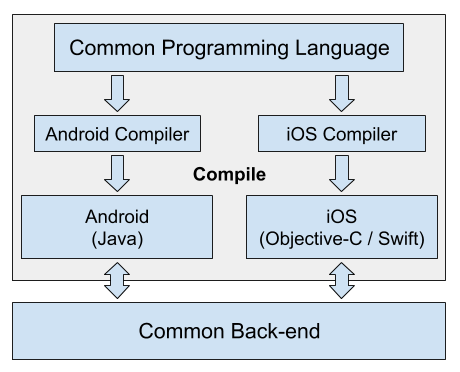
\includegraphics[width=0.5\linewidth]{PICs/Cross-Compiled.png}
\caption{Cross-compiled approach for Android and iOS \cite[p.~3]{7479278}}\label{Fig1}
\end{figure}
As a result of executing the native code compiled by the cross-compiler directly on the mobile device, this approach has almost the same performance as native applications. Through the use of a common programming language and the cross-compilers, each hardware feature can be accessed. However, certain features like camera access, location services, local notifications, etc., cannot be shared between platforms, as each of those features have to be implemented for each supported platform \cite[p.~627]{6420693} \cite[p.~3-4]{7479278}. A possible solution based on this approach is Xamarin \cite[p.~3]{7934674}, which will be described in detail in Chapter 3 and was selected to showcase a comparison between technologies using this approach and the interpreted approach.

\subsection{Interpreted Approach}
In this approach, as shown in Figure \ref{Fig3}, code written in a common language (JavaScript, e.g.) which is interpreted and thereby generates equivalents of native components \cite[p.~3]{7479278}. The interpreter is supplied with the application and interprets the code at runtime. In order to have access to hardware functions, the interpreted application communicates with an abstraction layer \cite[p.~3]{7479278} \cite[p.~2]{7934674}.
\begin{figure}[!htbp]
\centering
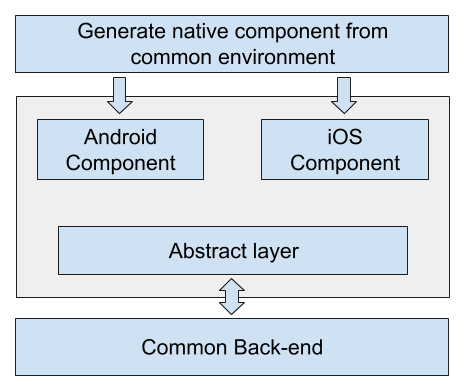
\includegraphics[width=0.5\linewidth]{PICs/Interpreted.png}
\caption{Interpreted approach for Android and iOS \cite[p.~3]{7479278}}\label{Fig3}
\end{figure}
Hardware features can be accessed through special Framework APIs, which simplifies the implementation of a component that requires them. Since native components are generated directly from the common language, the look and feel of the platform on which the application is executed is guaranteed. Despite JavaScript, which is also used in hybrid and web approaches, the interpreter does not require a browser or browser engine, which compared to the previously mentioned approaches leads to an improved performance \cite[p.~627]{6420693} \cite[p.~3]{7479278}. Technologies using this approach are Appcelerator Titanium (Axway, Santa Clara CA) and React Native \cite[p.~2]{7934674} \cite[p.~3]{JohanssonSderberg2018}. React Native will be discussed in more detail in the following chapters as it is selected for a comparison of technologies based on this approach with one based on the cross-compiled approach.

\subsection{Model Driven Approach}
The basis for this approach is provided by the Model Driven Architecture of the Object Management Group. The developer creates models with the functionality required for the application. These models are referred to as Computational Independent Models. As shown in Figure \ref{Fig2}, these undergo several transformations to yield platform specific source code that is able to communicate with the common back-end (e.g. business logic, data processing, data management). At first the created models are transformed into Platform Independent Models (PIM). These are then converted to Platform Specific Models (PSM) through the model-to-model transformation. PSMs are, as the name implies, different for each platform and are ultimately transformed into platform-specific source code through a model-to-text transformation. This model-to-text transformation consists normally on a template-based approach \cite[p.~4]{7479278} \cite[p.~3]{7934674}.
\begin{figure}[!htbp]
\centering
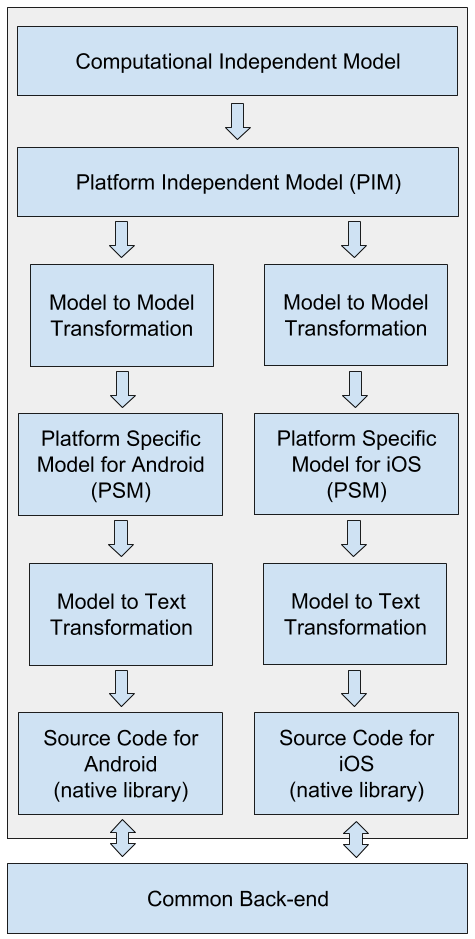
\includegraphics[width=0.5\linewidth]{PICs/MDA.png}
\caption{Transformation from model to source code for Android and iOS \cite[p.~4]{7479278} \cite[p.~3]{7934674}}\label{Fig2}
\end{figure}
\\[\baselineskip]
The problem with this approach is that so far, no mature framework is based on it. As a result, the full potential of this approach has yet to be demonstrated. Therefore, papers regarding the advantages and disadvantages of this approach are rare. However, a prototype framework called MD2 \cite{MD2} already exists, but since it is still relatively young and no official version was released till now, its usage and reliability for proper analysis are still limited \cite[p.~3-4]{7934674}.

\chapter{Selected Frameworks}
As this paper focuses on presenting a comparison between technologies using either the cross-compiled or interpreted approach, at least two frameworks to compare with each other had to be chosen. The selected ones are Xamarin and React Native, although theoretically more frameworks could have been selected. However, working with more than one technology per approach would lead to comparing the implementations of the same approach with each other which is not the aim of this thesis. 
\\[\baselineskip]
Though selecting exactly two frameworks does not completely eliminate the possibility of only comparing two implementations with each other that just used a different approach as a solution. Furthermore, if one of these frameworks had a bad implementation, it could lead to far worse results than the other framework using the same approach could achieve. This is why the selected frameworks have to be of high quality, but testing every known cross-platform framework would have exceeded the scope of this thesis, so lots of researching for related work had to be done. 
\\[\baselineskip]
The biggest reasons for selecting Xamarin and React Native were that both support Android and iOS \cite[p.~1]{JohanssonSderberg2018} \cite[p.~12]{ZubaBernhard2017EdPb}, that both still get new features, bug fixes and improvements \cite{XamarinRoadmap} \cite{ReactNativeRoadmap} and a good amount of valuable studies were available to work with (\cite{Danielsson_2016}, \cite{MartinezLecomte2018}, \cite{GaouarBenamarBendimerad2016} e.g.).

\section{Xamarin}
With the idea of developing a cross-platform framework that allows writing an application running on iOS, Android, Windows (Microsoft Corporation, Redmond WA) and MacOS (Apple Inc., Cupertino CA), the company Xamarin was founded in May 2011. The resulting framework called Xamarin offers the possibility to create a project in which C\# can be used as a programming language to develop a cross-platform application. If hardware features unable to be implemented via common code are required, platform specific C\#-code can be written into the project of the respective platform in order to enable implementation of the feature in said platform. Xamarin was bought by Microsoft in 2016 and is since then included in every version of Visual Studio \cite[p.~14]{ZubaBernhard2017EdPb} \cite[p.~16]{LinckArne2016}.
\\[\baselineskip]
The basis of Xamarin is the Mono framework, which is an open source implementation of the C\# compiler and the Microsoft .NET framework. Its source code is compiled in bytecode (intermediate language) and then executed by the common language runtime (CLR), also called Mono runtime. In addition, the Mono runtime provides access to an ECMA (European Computer Manufacturers Association) common language infrastructure (CLI), a just-in-time compiler (JIT) and an ahead-of-time compiler (AOT) \cite[p.~14]{ZubaBernhard2017EdPb}.
\\[\baselineskip]
In order to successfully run an application developed with Xamarin on a mobile device that uses Android, the application must be compiled in bytecode (intermediate language). It is then packed together with the Mono runtime and installed on the device. If the application is now executed, both the Android runtime (ART) and the Mono runtime run simultaneously. During execution, the Mono Runtime uses its just-in-time compiler to compile the intermediate language to a native assembly. An exchange between the two runtimes is necessary if native functionalities or Java libraries need to be called. The communication between the two runtimes is handled by the Java Native Interface \cite[p.~14-15]{ZubaBernhard2017EdPb} \cite[p.~456]{WillocxVossaertNaessens2015}. Since iOS does not allow generation of code at runtime, the mono-framework's ahead-of-time compiler is used to translate the application's C\# code into native ARM assembler code. This will allow the application to run on iOS\cite[p.~15]{ZubaBernhard2017EdPb} \cite[p.~456]{WillocxVossaertNaessens2015}.
\\[\baselineskip]
When generating a Xamarin project, it is possible to created it as either a Portable Class Library (PCL) or a Shared Asset Project (SAP). Both choices allow you to share the common code. The difference is that with PCL, the shared code is packaged into a dynamically-referenced library and then integrated into the various platforms at the runtime of the application. However, with SAP, the common code is already included in the respective projects when the application is built. According to Microsoft, developers should use PCL \cite[p.~16]{ZubaBernhard2017EdPb} \cite[p.~8-9]{Dickson_2013}.
\\[\baselineskip] 
In order to support platform-independent user interfaces with Xamarin, Xamarin.Forms was invented in 2014. When Xamarin.Forms is used, one or more XAML (extensible application markup language) files must be created in which the user interface controls can be defined. During compilation, each XAML file is translated into a BAML (binary application markup language) file, which provides the basis for reusing the user interface across multiple platforms. Then, each defined user interface control is mapped to the respective native counterpart. However, as a result only those user interface controls available on all platforms can be defined \cite[p.~17-18]{ZubaBernhard2017EdPb}.

\section{React Native}
With the words "learn once, write anywhere" Facebook announced its cross-platform framework, React Native, at the F8 conference in March 2015 \cite[p.~10]{Danielsson_2016} \cite[p.~21]{ZubaBernhard2017EdPb}. React-Native, which uses the JavaScprit library React as basis, provides the ability to use JavaScript to develop native applications for Android and iOS. For rendering an application using React Native, no browser is required.Instead the application runs on Android and iOS in a JavaScriptCore VM \cite[p.~10]{Danielsson_2016} \cite[p.~28]{ZubaBernhard2017EdPb}. In addition, hosting the application and transfering the computation of the layout to a thread other than the main thread dors not require a WebView container or browser. This makes it possible to develop applications with native responsiveness \cite[p.~10-11]{Danielsson_2016}.
\\[\baselineskip]
Like React Native, React was developed by Facebook, but not in order to enable cross-platform development but to simplify the presentation of complex user interfaces \cite[p.~8]{Danielsson_2016}. React makes this possible by on the one hand, dividing the complete user interface into so-called components, and on the other hand by the fact that for each imaginable condition of the user interface a state is defined. The user is then presented with one of these states for each component of the user interface. Depending on the interaction with the user or by receiving data via a web service, these states change \cite[p.~8-9]{Danielsson_2016} \cite[p.~21-27]{ZubaBernhard2017EdPb}. To enable a high-performance reload of the various states, React uses a virtual DOM (document object model). This is an abstraction of the real DOM which only serves is to assist React by rendering a new virtual DOM, when changes to the data model of a state occur. This result is then compared to the previous virtual DOM and the differences between the two are identified. As a result, only the minimal number of elements in the real DOM have to be reloaded \cite[p.~8-9]{Danielsson_2016}.
\begin{figure}[!htbp]
\centering
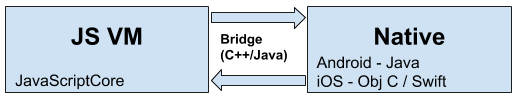
\includegraphics[width=0.75\linewidth]{PICs/Bachelor1_NativeBridge.png}
\caption{Native Bridge for Android and iOS \cite{PicReactNativeBridge} \cite[p.~28]{ZubaBernhard2017EdPb}}\label{Fig4}
\end{figure}
To enable communication between the native code, the native interface, and the JavaScript code, a so called Native Bridge was invented. In this concept, as shown in Figure \ref{Fig4}, data is transmitted via a C++ or Java bridge \cite[p.~28]{ZubaBernhard2017EdPb}. How exactly the data transfer of the JavaScript virtual machine with the respective operating system takes place, is defined in a protocol created by Facebook. To keep the transmission of information as short as possible, the protocol was kept slim \cite[p.~9-10]{Hansson_Vidhall_2016} \cite[p.~28]{ZubaBernhard2017EdPb}. Basically, if a method has to be called by the other party, a method with the same name as the required method is called and the parameters are passed. If a party has to call several methods of the other party, they are collected and then transmitted together \cite[p.~29]{ZubaBernhard2017EdPb}.

\newpage
\chapter{Evaluation}
This chapter deals in detail with the cross-platform frameworks Xamarin and React Native in comparison to native technologies. In addition, the following chapters are used to answer the research questions asked at the beginning. For both frameworks, studies that dealt with the criteria explained were selected for this chapter. Lastly, the results of the respective studies are presented.

\section{Criteria}
This section explains why the criteria of performance, code sharing, documentation and look and feel were chosen to evaluate the potential of Xamarin and React Native. Furthermore, for each criterion, a description is given as to whether the presented results of the selected studies directly dealt with Xamarin and React Native in their experiments or whether only results to one of the two frameworks exist. At the end, the papers used are listed for each criterion and briefly summarized.

\subsection{Performance}
While researching for papers that dealt with either Xamarin or React Native or both frameworks, almost all authors had something to say about the performance of the framework in question and it quickly became clear that one of the criteria under consideration had to be performance. Another reason was that when choosing a framework for developing a new application often the one with the best performance is chosen. Unfortunately, cross-platform frameworks have a bad reputation in terms of performance, which often leads to selecting native frameworks at the end. To find out if Xamarin and React Native deserve this bad reputation, studies conducting the same experiment with both technologies were picked for this criterion. The following paper was used: Bernhard Zuba compares Xamarin and React Native with native Android and iOS. The experiment in question focuses on measuring performance of a bubble-sort algorithm implemented with each technology \cite[p.~30-32]{ZubaBernhard2017EdPb}.

\subsection{Code Sharing}
This criterion was chosen to find out how much code a cross-platform framework such as Xamarin or React Native really shares across all platforms. Especially for this criterion, it was important to find results on experiments that were carried out on both Xamarin and React Native, since they had little significance without comparison, unlike the results of the other three criteria. The following paper was used for this criterion: In this experiment, Bernhard Zuba compares Xamarin and React Native in terms of the amount of code that can be shared across different platforms. The task to be fulfilled is to port an existing web app into a native application \cite[p.~71-73]{ZubaBernhard2017EdPb}.

\subsection{Documentation}
The purpose of this criterion was to get an idea of how difficult it is to start developing crossplatform applications with either Xamarin or React Native. However, while researching into studies on Xamarin and/or React Native regarding how good or bad the official documentation is, little to no studies were found. The only time authors wrote about the documentation was when they experimented with developing a cross-platform application with either React Native, Xamarin or both. The information contained in those experiments consists mostly of explanations as to how the documentation has helped them to solve problems or which information was missing in the official documentation. Some examples of this theses and papers are as follows:
\begin{itemize}
\item Developing a React Native application \cite[p.~16-18]{Danielsson_2016}
\item Developing a geo location and a Bluetooth feature, a shared library and creating native bindings for a Xamarin cross-platform application \cite[p.~10-15]{Dickson_2013} 
\item Porting a HTML5 web application to a React Native cross-platform application and a Xamarin cross-platform application \cite[p.~33-69]{ZubaBernhard2017EdPb}.
\end{itemize}
These circumstances led to a change of purpose for this criterion. Prior, the aim was to compare the official documentations of Xamarin and React Native with each other and finding out if their respective documentation is missing important information. Now the objective is to summarize which experiences developers of React Native and Xamarin cross-platform applications had with using the official documentation of either Xamarin or React Native.

\subsection{Look and feel}
In the beginning this criterion was chosen to find out if Xamarin and React Native adhere to the OS user interface guidelines, however, most studies found that discuss this topic concentrated on the user experience and did not mention anything about OS guidelines. Therefor the goal of this criterion was changed to finding out if mobile application users notice a difference between the look and feel of native applications compared to cross-platform applications created with Xamarin or React Native. Since this criterion is not easily measurable, most authors rely on questionnaires or interviews. Again, like the problem in regard to Documentation, no study could be found that performs the same experiment for both Xamarin and React Native. Which is why more emphasis is placed here on summarizing the results of studies, which will be discussed later in this paper. For React Native alone, several studies on look and feel could be found quickly, which meant that only one had to be chosen. However, problems arose, as hardly any papers made experiments on the look and feel of Xamarin. The few sources found pointed out, that due to Xamarin's cross-compiled approach, the look and feel of the application was, in general, authentic, at least, when Xamarin.Forms is used for developing the UI. The studies used for this criterion are the following:
\begin{itemize}
\item Defining desirable criteria for cross-platform frameworks by summarizing results from studies on existing cross-platform frameworks\cite[p.~21]{GaouarBenamarBendimerad2016} \cite[p.~8]{tunali2015comparison}
\item Replicating an Android application with React Native and comparing the look-and-feel by consulting 25 people \cite[p.~16-18]{Danielsson_2016}
\end{itemize}

\section{Results}
The following chapters showcase and discuss the results of studies and experiments regarding the two cross platform mobile development frameworks Xamarin and React Native. Whenever possible, studies which underwent experiments with both frameworks were chosen. Additionally, several other noteworthy studies which only underwent experiments with one of the two frameworks are also featured. While the results of these studies are not comparable with each other, not including them ignore interesting data on the aforementioned criteria. By incorporating these studies, one gains a better picture of Xamarin and React Native in respect of performance, code sharing, documentation and look and feel. The studies, which used both frameworks for their experiments, also provided comparisons and discussions of the results. These comparisons and discussions are also summarized in the following chapters.

\subsection{Performance}
In his work \cite{ZubaBernhard2017EdPb}, Bernhard Zuba compared the performance of a native Android and iOS application with that of a React Native and Xamarin application. With each technology the same bubble-sort algorithm was implemented and then while sorting the elements the performance per application was measured \cite[p.~30]{ZubaBernhard2017EdPb}. According to Zuba, the native application with the Xamarin application is pretty much the same on Android. The same applies to the React Native application up to 1000 elements, but its performance drops sharply thereafter \cite[p.~30]{ZubaBernhard2017EdPb}. The measurements in the iOS applications give a very similar picture as before. Here, too, the performance of the React Native application drops again from 1000 elements. 
\\[\baselineskip]
The results of the native application and the Xamarin application were very similar if the number of elements was low. But when using 20000 elements, the native application takes twice as long. Zuba suspects that the reason for the better performance of the Xamarin application is due to the code optimization of Xamarin, which Xcode (Apple Inc., Cupertino CA) may have not done \cite[p.~31]{ZubaBernhard2017EdPb}. In the end, Zuba believes that both the Xamarin and the React Native applications can keep up with the native applications. Furthermore, he points out that in practice, if a mobile application uses a large number of elements, these are usually sorted and edited on the server side. This would allow React Native applications to compete with native applications as well. If, however, a requirement for the application were to have very good performance, for example, if many complex arithmetical operations had to be performed, Xamarin would be a better choice than React Native. Another alternative, according to Zuba, is to write native code for such operations and then integrate it into Xamarin or React Native on the respective platform \cite[p.~32]{ZubaBernhard2017EdPb}.

\subsection{Code Sharing}
In his master thesis \cite{ZubaBernhard2017EdPb}, Bernhard Zuba ported a web app as a native application once using Xamarin and once using React Native. The tool sloc (NPM Inc., Oakland CA) was used to count the lines of code. In Xamarin, the business logic could be shared to 100\% across all platforms, only platform-specific code had to be written for the initialization of a SQLite database – 19 lines of code for Android and 23 for iOS. Basically, everything could be shared in the UI, but in order to match the style guide, it was necessary to create custom components because there were too many limitations with Xamarin. Here, 1888 lines of code could be shared across the platforms, 243 lines of platform-specific code had to be written for Android and 168 lines of platform-specific code for iOS \cite[p.~71]{ZubaBernhard2017EdPb}. For the React Native application, a total of 2725 lines of code for business logic and UI were written, all of which are 100\% cross-platform, but the Xamarin application is smaller by 167 lines of code. Since the web app consisted largely of JavaScript, Zuba could reuse 804 lines of code for the React Native application \cite[p.~72]{ZubaBernhard2017EdPb}. In conclusion, Zuba comments that in this experiment both frameworks were nearly perfect, yet React Native outperformed Xamarin \cite[p.~72-73]{ZubaBernhard2017EdPb}.

\subsection{Documentation}
The first part of this chapter showcases the results of the papers concerning the official documentation of React Native , followed by those of Xamarin. All other possible sources for information regarding Xamarin and React Native are listed in the latter part of this chapter. 
\\[\baselineskip]
The following list includes the experiences William Danielsson had with the documentation of
React Native \cite{ReactNativeDoc} while experimenting on developing a replication of an Android application with React Native: 
\begin{itemize}
\item Through following the steps of the documentation’s chapter "Getting Started", William Danielsson was able to set up the development environment for Android and iOS regarding the operating system used on his computer, connect to a physical mobile device, set up a virtual mobile device and create a new project without having a problem \cite[p.~18]{Danielsson_2016}.
\item When trying to implement a feature that captures a photo with the camera of the mobile device, multiple errors occurred. One of the problems William Danielsson had to face was that React Native did not support a component for the camera at the time of his experiment. However, Lochlan Wansbrough, a creator of many React Native components, created an open-source camera component. This components repository \cite{ReactNativeCamera} is now part of the official React Native community account \cite{ReactNativeCommunity}. The second problem William Danielsson had was that the documentation of this component only existed for iOS and not for Android. He stated that the feature was not implemented for Android because it would have exceeded the scope of his experiment \cite[p.~23-24]{Danielsson_2016}.
\item For the same functionalities as in the original application to be offered by the React Native application, it must also be possible to switch from one activity to another. However, as React Native’s official documentation did not provide enough information for William Danielsson, he had to access other sources. He solved this problem by consulting the following blog
\cite[p.~51]{Danielsson_2016} \cite{ReactNativeBlog}.
\end{itemize}
Jared Dickson’s master thesis deals with mobile development with Xamarin, which is why his experiment was based on developing a geo location, a Bluetooth feature, a shared library and creating native bindings for a Xamarin application by using the official documentation of Xamarin \cite{XamarinDoc} as a source. However, as he was developing the Bluetooth feature which should have sent messages from one device to another via a Bluetooth connection, he found out, that the documentation for implementing a feature using Bluetooth connection on iOS was nonexistent. The experiment was finished without implementing this feature for iOS. He states however, that at the time he was writing his thesis "Core Bluetooth" was released which allows access to the Bluetooth feature on iOS and would have solved his problem \cite[p.~11]{Dickson_2013}.
\\[\baselineskip]
By analyzing a two-page Q\&A Matias Martinez and Sylvain Lecomte tried to find out more about the documentation of Xamarin's error codes. The data for this study was gathered by roaming through all questions asked on the Xamarin Forum and on Stack Overflow, which contained an error code thrown by the Xamarin framework. Martinez and Lecomte found a total of 1121 and 330 questions (on the Xamarin Forum and Stack Overflow respectively) including at least one Xamarin error code. 87.5\% of the questions on the Xamarin Forum and 92.3\% of the questions on Stack Overflow were answered. With this information, they now plan to analyze these answers and summarize the results to further help developers find a solution for their problem with Xamarin as fast as possible \cite[p.~1,~4]{MartinezLecomte2018}.
\\[\baselineskip]
At last, most authors of these or similar studies, papers or theses have mentioned where they also searched for information during their experiments. Their sources will be summarized here. The official documentations of Xamarin and React Native are not the only ways to get detailed information regarding the specific framework. Like Martinez and Lecomte, most developers also used StackOverflow as a source for explanations and code examples \cite{MartinezLecomte2018}. When searching for solutions or information regarding a problem with the native code Xamarin and React Native, developers can also revert to the official documentations of Android and iOS \cite[p.~11]{Dickson_2013}. More possible sources for information are included in React’s documentation for React Native developers \cite{ReactDoc} and in the Xamarin Forum for Xamarin developers \cite[p.~51]{Danielsson_2016} \cite{MartinezLecomte2018}.

\subsection{Look and feel}
Danielsson replicated an Android application with React-Native for his paper \cite{Danielsson_2016}. To compare the look and feel of the React-Native with the Android application, he shared the two applications with 25 consultants. Each consultant had to answer three questions in regard to the application given to them. But, with the exception of the last question, Danielsson would not tell the consultants which application they were using and gave them no limitations what they were allowed to do with them \cite[p.~29]{Danielsson_2016}. The first question was which application the React Native application is, the second one how confident the subject is with their answer to the first question and the third question was if after using both applications and seeing them in action compared to each other, the subject still would like to use a React Native application in the future \cite[p.~29-31]{Danielsson_2016}. In conclusion, 18 subjects were able to distinguish the two applications, while 7 were not able to do so with certainty \cite[p.~30]{Danielsson_2016}. 12 of the 18 said, that they were "positive" with their answer. The remaining 6 said they were "pretty sure". As a reason why they chose which application is the React Native application, most of the 12 subjects who chose "positive" said the animation of the transitions from one screen to another was unknown to them which made them suspicious. Most of the 6 subjects who chose "pretty sure" said that they assumed the application with the longer start-up-time was the React Native application \cite[p.~30]{Danielsson_2016}. Out of all 25 test persons, 24 said that they would also use React Native applications next to native applications in the future \cite[p.~31]{Danielsson_2016}. The author concludes from these results that although the React Native application was slightly slower than the native Android application and the transitions from one screen to the other had a different animation, almost all subjects had no problem using the application. Despite the fact the React Native application lagged behind in this test, it was not nearly enough that it would deter or limit users in anyway \cite[p.~45]{Danielsson_2016}.
\\[\baselineskip]
In the work of Tunali and Erdogan \cite{tunali2015comparison} as well as in the paper of Gaouar, Benamar and Bendimerad \cite{GaouarBenamarBendimerad2016}, the authors try to summarize all desirable criteria that a cross-platform framework should have, based on studies of existing frameworks. One of these criteria is look and feel. For Xamarin, though, it is often pointed out that in terms of look and feel, prior to the release of Xamarin.Forms, developing the UI took some time because for each platform a new UI had to be designed, but no comparison regarding the look and feel prior to the release of Xamarin.Forms with native applications was made \cite[p.~20]{GaouarBenamarBendimerad2016} \cite[p.~5]{tunali2015comparison}. As for the period after the release of Xamarin.Forms, in both of the aforementioned papers the look and feel of Xamarin is equated with that of an application developed with platform-specific technologies. The reason that both papers state this is the cross-compiled approach of Xamarin, which translates every UI component defined in Xamarin.Forms as a native component  \cite[p.~21]{GaouarBenamarBendimerad2016} \cite[p.~5,~8]{tunali2015comparison}.

\newpage
\chapter{Conclusion \& Future Work}
The aim of this work was to give a better picture of the potential of cross-platform frameworks for mobile Android and iOS application development. All known mobile development approaches were presented in terms of their strengths and weaknesses.
\\[\baselineskip]
In particular, the development approaches cross-compiled and interpreted were discussed. For each of these approaches, a framework was chosen that uses the same approach, in this case Xamarin and React Native. These were then compared using studies that focused on performance, code sharing, documentation and look and feel. The evaluation attempted to answer the research questions presented in the introduction, although this turned out to be more difficult than initially expected. One of the main reasons for the difficulties that arose was the fact, that only a handful of studies using both Xamarin and React Native in their experiments, existed in the first place. This meant that a direct comparison between the two frameworks and therefore between the cross-compiled and the interpreted approach was difficult.
\\[\baselineskip]
Another problem was that answering the last research question was not entirely possible. The studies researched for the look and feel criterion focused more on analyzing the user experience of the particular application rather than evaluating the operating systems user interface policies.
\\[\baselineskip]
Overall, however, it turned out that cross-platform frameworks do not lag behind platform-specific frameworks in terms of their overall efficiency. The performance criterion even showed that the cross-compiled Xamarin application even surpasses the platform-specific application in compute-intensive operations. Xamarin and React Native have a lot of room for improvement mainly with the criterion documentation, therefore extending the documentation of both frameworks could be chosen as a future goal. Another possible goal would be to pay more attention to operating system user interface policies to find out, if implementing these policies in cross-platform frameworks becomes necessary for future mobile application development.




% Hier beginnen die Verzeichnisse.
\clearpage
\ifthenelse{\equal{\FHTWCitationType}{HARVARD}}{}{\bibliographystyle{gerabbrv}}
\bibliography{Literatur}
\clearpage

% Das Abbildungsverzeichnis
\listoffigures
\clearpage

\phantomsection
\addcontentsline{toc}{chapter}{\listacroname}
\chapter*{\listacroname}
\begin{acronym}[XXXXX]
    \acro{iOS}[iOS]{iPhone Operating System}
    \acro{OS}[OS]{Operating System}
    \acro{CPU}[CPU]{Central Processing Unit}
    \acro{GPU}[GPU]{Graphics Processing Unit}
    \acro{SDK}[SDK]{Software Development Kit}
    \acro{API}[API]{Application Programming Interface}
    \acro{ECMA}[ECMA]{European Computer Manufacturers Association}
    \acro{W3C}[W3C]{World Wide Web Consortium}
    \acro{HTML}[HTML]{Hypertext Markup Language}
    \acro{CSS}[CSS]{Cascading Style Sheets}
    \acro{VM}[VM]{Virtual Machine}
    \acro{DOM}[DOM]{Document Object Model}
    \acro{QnA}[Q\&A]{Questions and Answers}
    \acro{UI}[UI]{User Interface}
\end{acronym}

\end{document}}